%_____________________________________________________________________________________________ 
% A Holistic Approach to Autonomic Self-Healing Cloud Computing Architecture
% Chapter 3 - Existing Solutions
% Fri Apr 19 12:53:32 IST 2013
%_____________________________________________________________________________________________
\chapter{Existing Solutions}
% Add Citation
\section{Autonomic computing system with model transfer}
\textbf{Patent number:} 7542956\cite{STRASSNER:2009}\\
Different data and commands are received from different devices and they are sent to an autonomic manager to produce a single normalized view of the information. The actual state is identified from the normalized view which is compared to the desired state. If there is a difference, configuration adjustment is done to reach the desired state.
	\begin{figure}[h]
		\begin{center}
			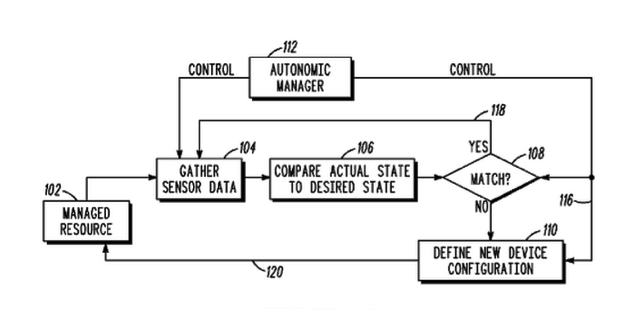
\includegraphics{figures/patent1_1.eps} 
			\caption{\small \sl Approach for Controlling a Managed Resource using an Autonomic System.\label{fig:Label1}} 
		\end{center} 
	\end{figure}

The technique uses machine learning, dependency processing and action determination logic to decide the action to be taken in case of a mismatch.
	\begin{figure}[h]
		\begin{center}
			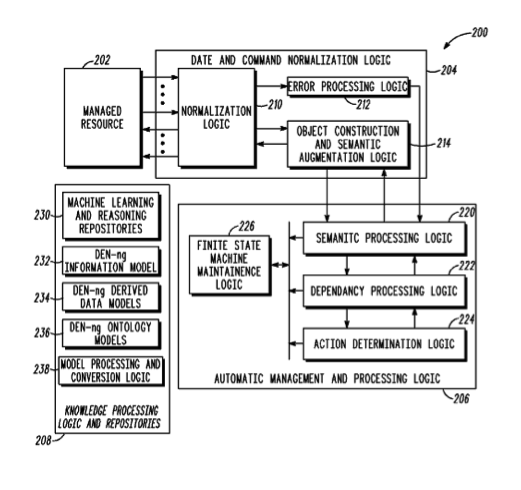
\includegraphics{figures/patent1_2.eps} 
			\caption{\small \sl Block diagram of an Autonomic System.\label{fig:Label2}} 
		\end{center} 
	\end{figure}
% Add Citation
\section{Architecture for a Self-Healing Computer System}
\textbf{Patent number:}  2010/0281134 (Patent pending)\cite{MELEN:2010}\\
The self healing system comprises a self healing processor and an error mitigation system, a code block associated with the operation of a portion of digital logic, dynamic signature analysis circuit. The processor executes the code block. The dynamic signature analysis circuit creates a dynamic signature representing the operation of the portion of digital logic associated with the code block. The error mitigation system receives the dynamic signature from the dynamic signature analysis circuit, and compares it with a static signature to determine if the signatures match. If the signatures do not match then the digital logic associated with the code block has an error. The error mitigation system retries execution of the code block. The error mitigation system stores log information describing the above events.
	\begin{figure}[h]
		\begin{center} 
			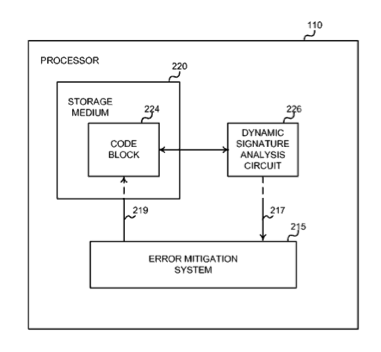
\includegraphics{figures/patent2_1.eps} 
			\caption{\small \sl Embodiment of a Self Healing Processor.\label{fig:Label3}} 
		\end{center} 
	\end{figure}

The Error Mitigation System is the core of the entire architecture. It houses a variety of components that help in finding out the error and correcting it. A lot of techniques like learning and lookup tables are used in this.
	\begin{figure}[h]
		\begin{center}
			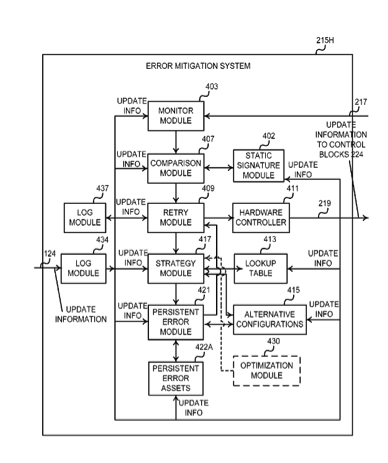
\includegraphics{figures/patent2_2.eps} 
			\caption{\small \sl Embodiment of an Error Mitigation System.\label{fig:Label4}} 
		\end{center} 
	\end{figure}

% Add Citation
\section{System and Method for Achieving Autonomic Computing Self Healing Utilizing Meta Level Reflection and Reasoning}
\textbf{Patent number:}  7260743\cite{FELLENSTEIN:2007}\\
In a base level a monitor detects an error in a production environment and provides reification message comprising data about the error to a meta level. A reasoning system in the meta level receives the reification message and analyzes the data using knowledge of computational components in the base level and identifies a self healing action for the error and returns a reversion message comprising a signal to implement the self healing action. Responsive to receiving the signal the base level implements the self-healing action.
	\begin{figure}[h]
		\begin{center}
			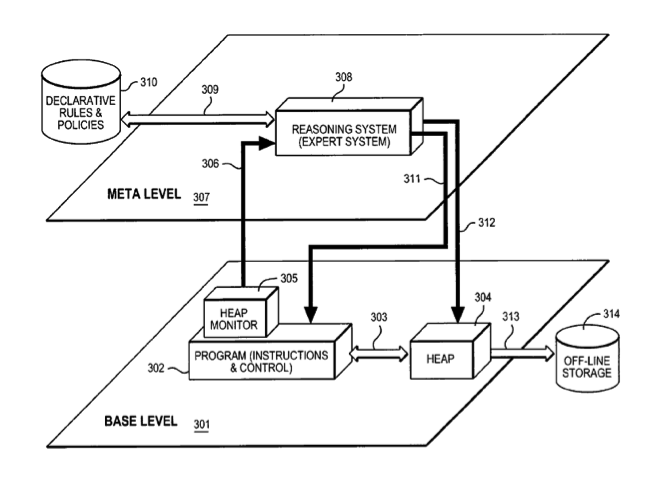
\includegraphics{figures/patent3.eps} 
			\caption{\small \sl System and method for Handling Errors.\label{fig:Label5}} 
		\end{center} 
	\end{figure}
\section{Comparison of the various approaches}
%\begin{table}		% Table
\begin{center}
\small		
%\begin{tabular}{| p{4cm} | p{4cm} | p{4cm} |}	% Format	
\begin{longtable}{| p{3cm} | p{3.5cm} | p{3.5cm} | p{3.5cm} |}
\hline 
\bf{Features} & \bf{Autonomic Computing System with Model Transfer } & \bf{Architecture for a Self Healing Computing System} & \bf{System and Method for Achieving Autonomic Computing Self Healing Utilising Meta Level Reflection and Reasoning}\\ \hline
{Comparison Parameters} & {Sensor State Comparison} & {Dynamic Signature Comparison} & {Reification Message} \\ \hline
{Separate Level used} & {No} & {No} & {Yes-Meta Level}\\ \hline
{Action Recommendation Logic} & {Learning based on creating models and mapping them to ontology includes semantic processing, dependency processing and action determination. } & {Static rules based. Uses Lookup table to map fault to strategy. Also has alternate configuration in case the basic strategy fails and a retry module. Strategy Optimisation is proposed not implemented.} & {Uses a reasoning system. Job is divided into two parts - detection (base level) and action recommendation (meta level). Transparency provided because of meta level.}\\ \hline
{Architecture specific requirements} & {Sensors} & {Error Mitigation System} & {Reasoning Expert System}\\ \hline
{Transparency} & {No} & {No} & {Yes- Multilevel}\\ \hline
{Feasibility} & {Excessive use of sensors. Too much of information collected, requires comparable hardware to process so much information.} & {Uses a specific processor that executes a code block and needs to interact with error mitigation system. Too much message passing} & {Meta level is idle most of the time. Fewer messages passed. Base level only sends messages when error is detected. Strategy can be easily decided and changed without modifications to the base level.}\\ \hline
{Dynamic Learning} & {Yes} & {No} & {Possible}\\ \hline
\caption{Comparison of the various approaches}
\end{longtable}
%\caption{A simple table: Test centuries}	% This will appear in List of Tables
\label{table1}
\end{center}
%\end{table}
%_____________________________________________________________________________________________ 

